\documentclass{article}
\usepackage[utf8]{inputenc}
\usepackage{amsmath}
\usepackage{amsfonts}
\usepackage{amssymb}
\usepackage{makeidx}
\usepackage{graphicx}
\usepackage{hyperref}
\usepackage{pdfpages}

\makeindex

%\usepackage{enumitem}
%\usepackage{subfigure}

\begin{document}
	
	
	\begin{titlepage}
		
		\newcommand{\HRule}{\rule{\linewidth}{0.5mm}} % Defines a new command for the horizontal lines, change thickness here
		
		\center % Center everything on the page
		
		%----------------------------------------------------------------------------------------
		%	HEADING SECTIONS
		%----------------------------------------------------------------------------------------
		
		\textsc{\LARGE Politecnico di Milano}\\[1.5cm] % Name of your university/college
		\textsc{\Large Design ed implementazione di un sito web}\\[0.5cm] % Major heading such as course name
	    %\textsc{\large Swift Ios}\\[0.5cm] % Minor heading such as course title
		
		%----------------------------------------------------------------------------------------
		%	TITLE SECTION
		%----------------------------------------------------------------------------------------
		
		\HRule \\[0.4cm]
		{ \huge \bfseries Progetto Hypermedia}\\[0.4cm] % Title of your document
		\HRule \\[1.5cm]
		
		%----------------------------------------------------------------------------------------
		%	AUTHOR SECTION
		%----------------------------------------------------------------------------------------
		
		\begin{minipage}{0.4\textwidth}
			\begin{flushleft} \large
				\emph{Autori:}\\
				Alessandro \textsc{Cimbelli} % Your name
				\\
				Matteo \textsc{Daverio} % Your name
				\\
				Mirko \textsc{Conti} % Your name
			\end{flushleft}
		\end{minipage}
		~
		\begin{minipage}{0.4\textwidth}
			\begin{flushright} \large
				\emph{Professore:} \\
				Franca \textsc{Garzotto} % Supervisor's Name
			\end{flushright}
		\end{minipage}\\[2cm]
		
		% If you don't want a supervisor, uncomment the two lines below and remove the section above
		%\Large \emph{Author:}\\
		%John \textsc{Smith}\\[3cm] % Your name
		
		
		%----------------------------------------------------------------------------------------
		%	LOGO SECTION
		%----------------------------------------------------------------------------------------
		
		
\includegraphics{Risorse/polimi.png}\\[1cm] % Include a department/university logo - this will require the graphicx package
		
		%----------------------------------------------------------------------------------------
		%	DATE SECTION
		%----------------------------------------------------------------------------------------
		
		
		{\large \today}\\[3cm] % Date, change the \today to a set date if you want to be precise
		
		
		%----------------------------------------------------------------------------------------
		
		\vfill % Fill the rest of the page with whitespace
		
	\end{titlepage}
	
	\tableofcontents
	
	\clearpage
	\section{Membri del gruppo}
	\begin{itemize}
		\item Alessandro Cimbelli: alessandro.cimbelli@mail.polimi.it
		\item Matteo Daverio: matteo.daverio@mail.polimi.it
		\item Mirko Conti: mirko1.conti@mail.polimi.it
	\end{itemize}
	
	\clearpage
	
	\section{Abstract}
	Il presente documento costituisce tutto il materiale di progettazione con il quale poi andremo ad implementare il sito web assegnatoci.
	La documentazione sarà organizzata secondo il seguente schema:
	
	\begin{enumerate}
		\item Diagrammi \emph{IDM} 
			\begin{itemize}
				\item \emph{C-IDM}
				\item \emph{L-IDM}
				\item \emph{P-IDM}
			\end{itemize}
			
			Nel P-IDM, per chiarire alcuni concetti, è stata inserita una legenda che spiega i nuovi simboli introdotti o eventuali chiarimenti.
	
		\item Mockup: Sviluppato attraverso Balsamiq. Nelle prossime righe verranno descritte le note relative al Mockup da tener presente in fase di valutazione:
		\begin{itemize}
			\item I link in alto a sinistra sono più di uno nonostante, in fase implementativa, sarà presente solo il link che porterà alla pagina precedentemente visualizzata. Questo è dovuto all'impossibilità di esprimere link dinamici attraverso il tool (Essi saranno contraddistinti da un asterisco).
			\item Alcuni link non sono funzionanti in quanto le pagine di destinazione sono strutturalmente identiche ad altre già presenti, ad esempio \emph{Tablet \& Computer} non è selezionabile essendo uguale a \emph{Smartphone \& Telefoni}.
		\end{itemize}
	\end{enumerate}
		
	\section{Features Aggiuntive}
		\begin{itemize}
			\item Menu a tendina che, come spiegato in classe, fornisce una versione alternativa di accesso ripetto a quanto rappresentato dal P-IDM.
			\item Implementazione di un filtro (indicato con F nel P-IDM nelle seguenti pagine):
				\begin{enumerate}
					\item Device by Category
					\item Promotion of Devices
					\item Correlated Devices
				\end{enumerate}
			\item Implementazione FAQ in SmartLife Services.
		\end{itemize}
		
	

	\section{Percorsi consigliati}
	Per facilitare la visita delle casistiche più intricate, consigliamo alcuni percorsi.
	\begin{itemize}
		\item $Assistance$ $Service \rightarrow Pagina$ $Intermedia \rightarrow Devices$
				\begin{enumerate}
					\item Servizi di Assistenza
					\item Supporto tecnico e configurazione
					\item Configurazione Mail su iPhone
					\item Vai a tutti gli iPhone
					\item Dettagli (Sull'iphone)
				\end{enumerate}
				
				Da qui si può ispezionare il path: $Devices \rightarrow Assistance$ $ Services$
				\begin{enumerate}
					\item Partendo sempre dall'iphone
					\item Scopri di più (Per scrollare la pagina)
					\item Vai al servizio (Tra i servizi di assistenza)
				\end{enumerate}
		\item $Assistance$ $Service \rightarrow Devices$
		\begin{enumerate}
			\item Servizi di Assistenza
			\item Supporto tecnico e configurazione
			\item Decoder Tim Vision
			\item Vai a Decoder Tim Vision
		\end{enumerate}
		
		\item $Smart$ $Life$ $Service \rightarrow Pagina$ $Intermedia \rightarrow Devices$
		\begin{enumerate}
			\item Dal menu a tendina di Smart Life Service selezionare \emph{Servizi alla Persona}
			\item Scopri (Pagamenti)
			\item Attivazione e regole
			\item Vai a dispositivi compatibili
			\item Dettagli (Sul Samsung Galaxy)
		\end{enumerate}
			Da qui si può ispezionare il path: $Devices \rightarrow Smart$ $ Life$ $ Services$
			\begin{enumerate}
				\item Partendo sempre dal Samsung Galaxy
				\item Scopri di più (Per scrollare la pagina)
				\item Vai al servizio (Tra gli smart life services)
			\end{enumerate}
			
		\item $Smart$ $Life$ $Service \rightarrow Devices$
		\begin{enumerate}
			\item Smart Life Services
			\item Tv \& Entertainment
			\item Scopri (Tim Vision)
			\item Attivazione e regole
			\item Scopri Smart Tv
		\end{enumerate}
	\end{itemize}

	\addtocounter{section}{1}
	\addcontentsline{toc}{section}{\arabic{section}~~Diagrammi}

		
		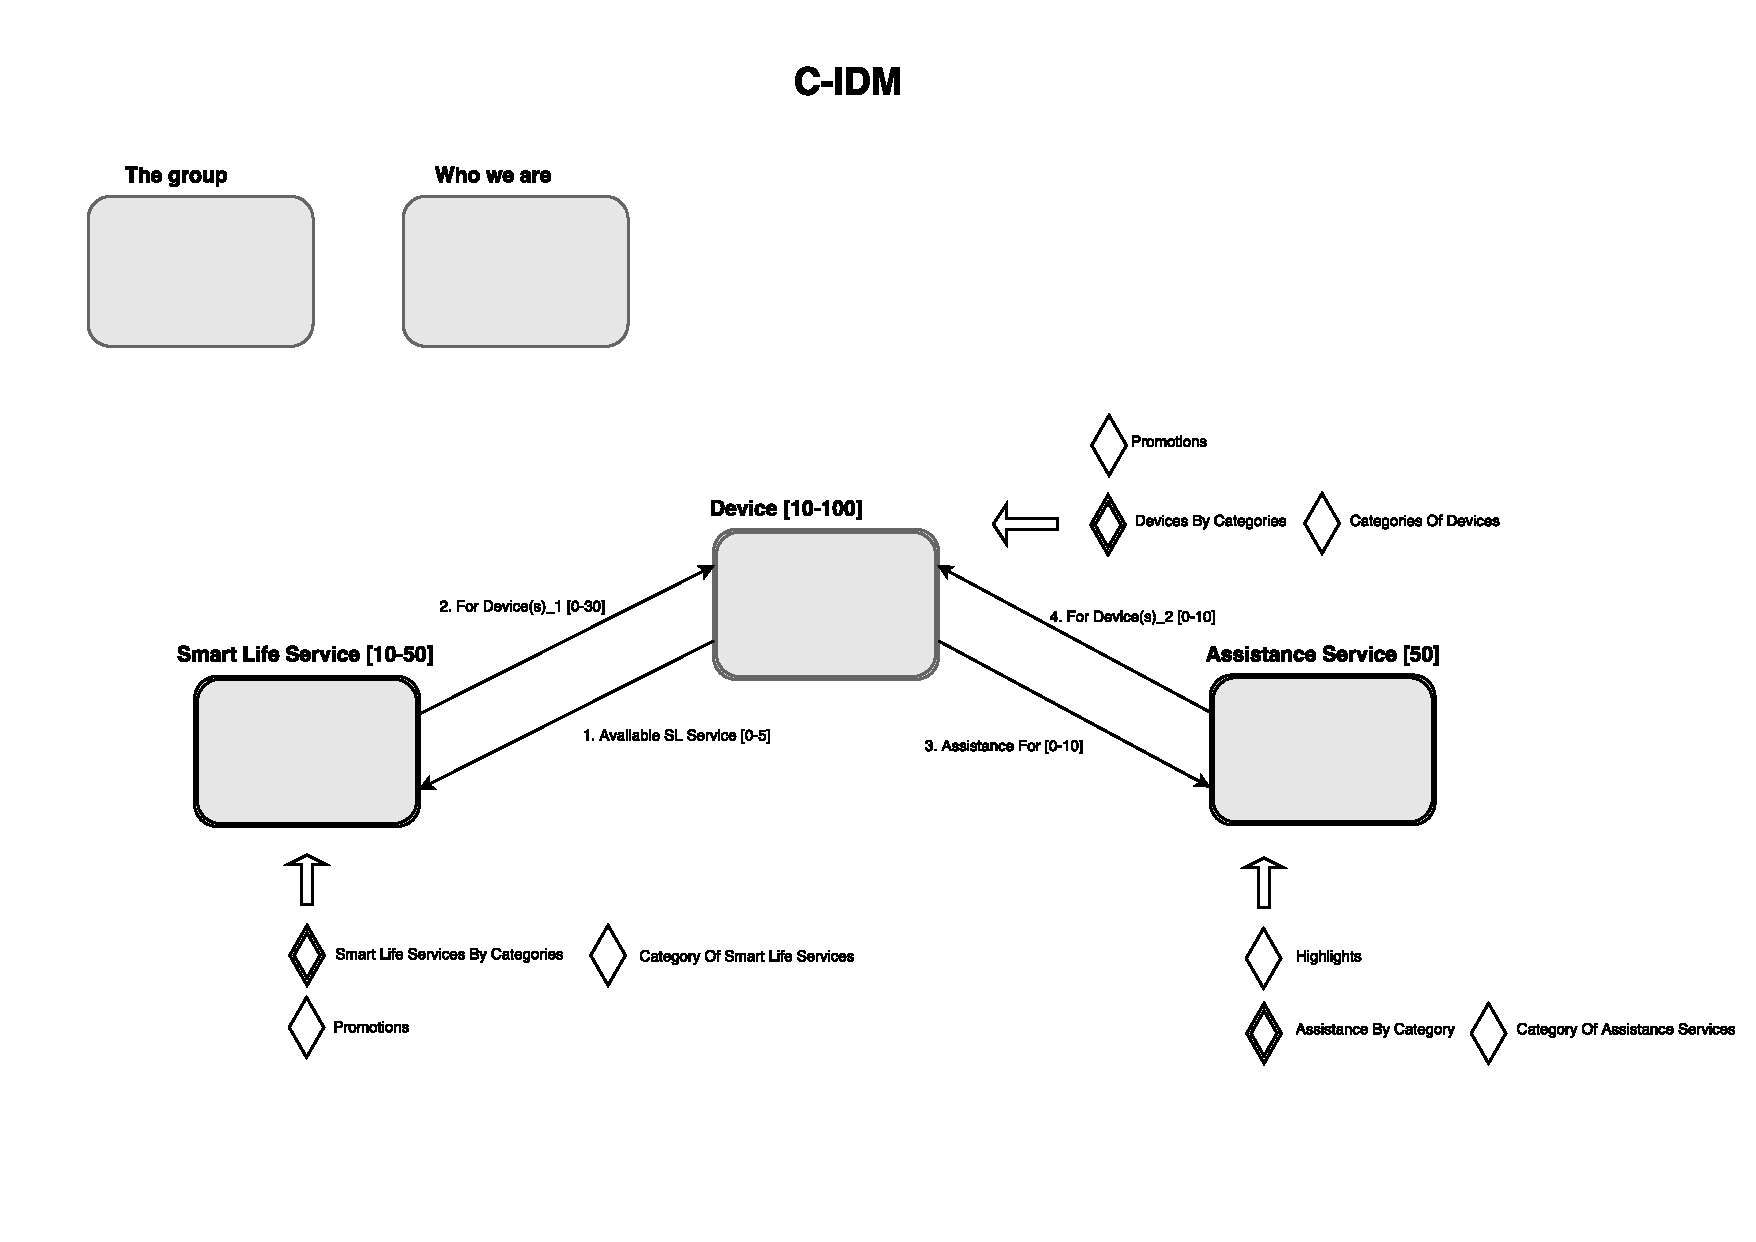
\includepdf[landscape=true, pagecommand={\thispagestyle{empty}
			\subsection*{}
			\addtocounter{subsection}{1}
			\addcontentsline{toc}{subsection}{\arabic{section}.\arabic{subsection}~~Diagramma C-IDM}}]{Risorse/C-IDM.pdf}

		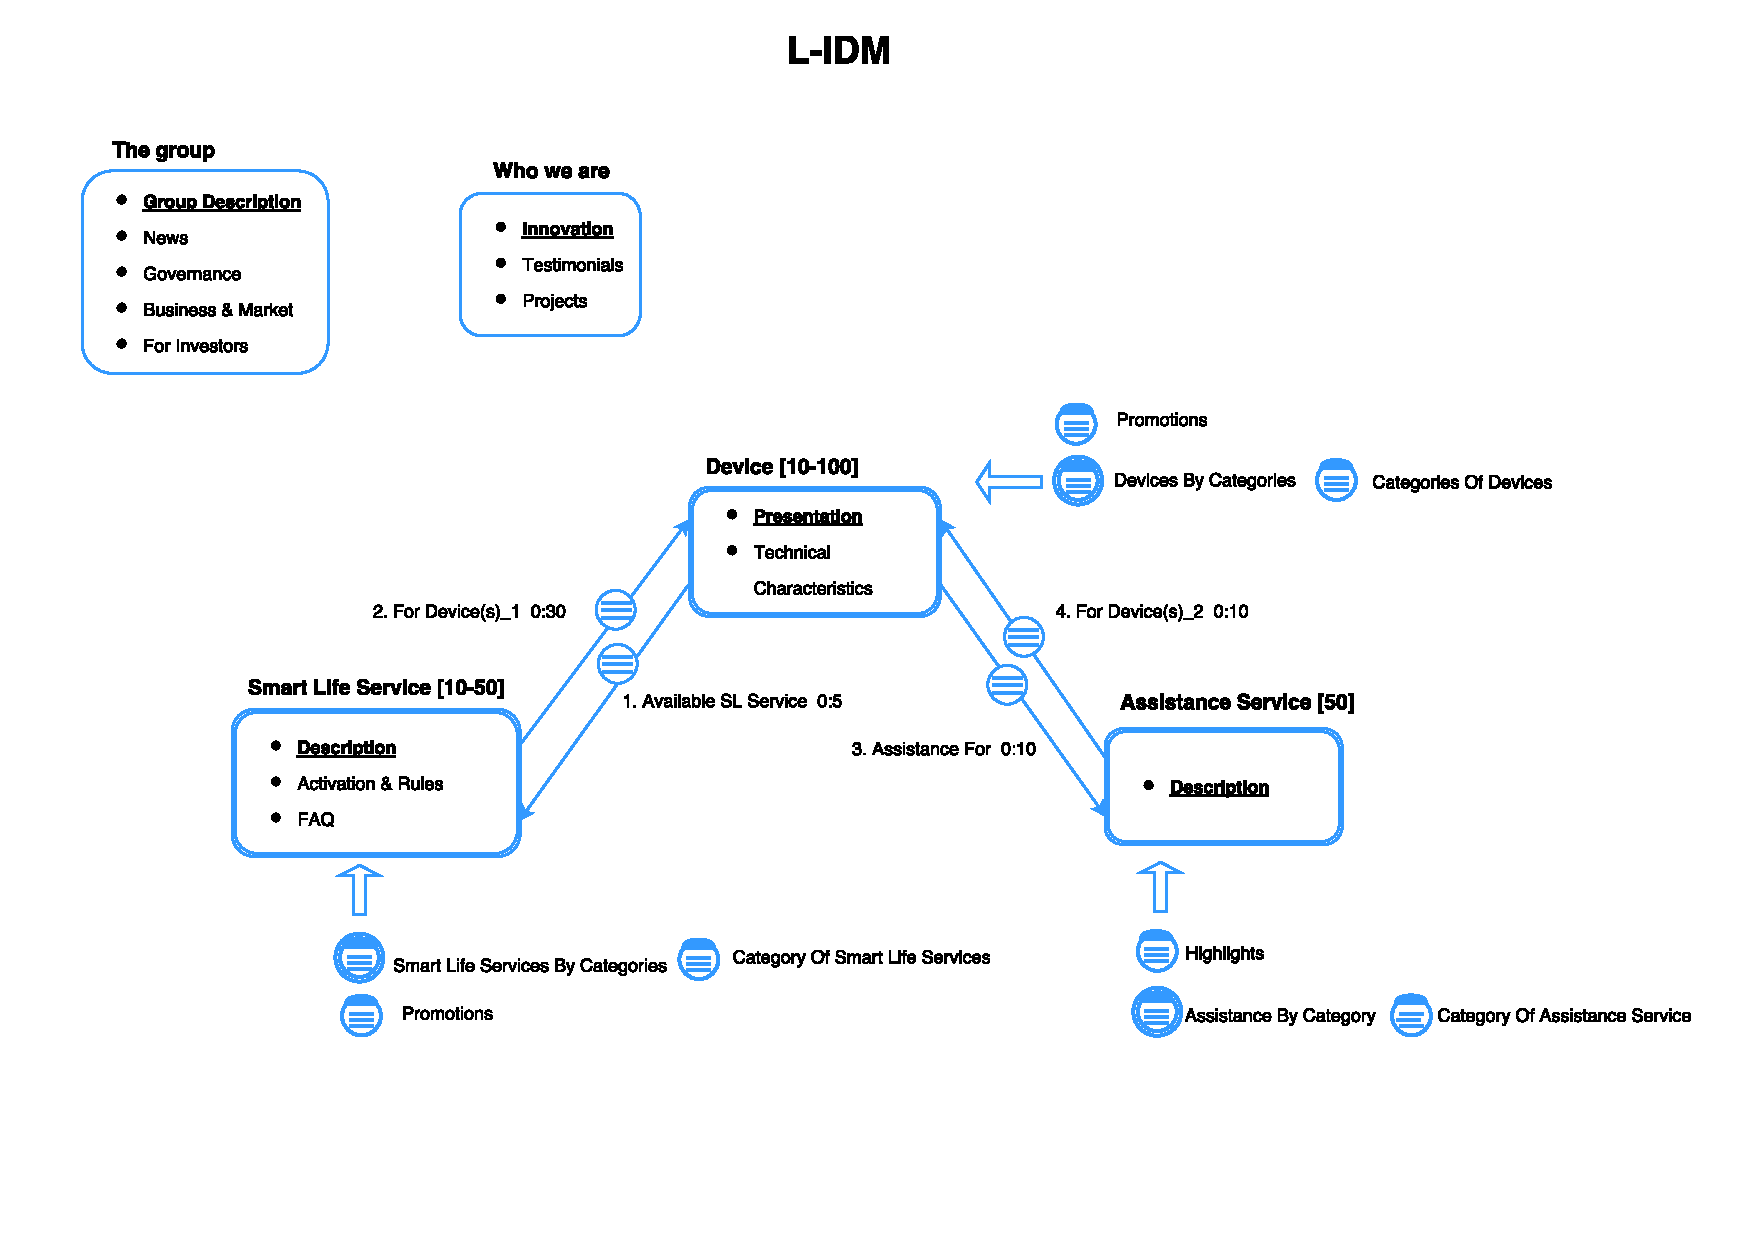
\includepdf[landscape=true, pagecommand={\thispagestyle{empty} \subsection*{}
			\addtocounter{subsection}{1}
			\addcontentsline{toc}{subsection}{\arabic{section}.\arabic{subsection}~~Diagramma L-IDM}}]{Risorse/L-IDM.pdf}
		
		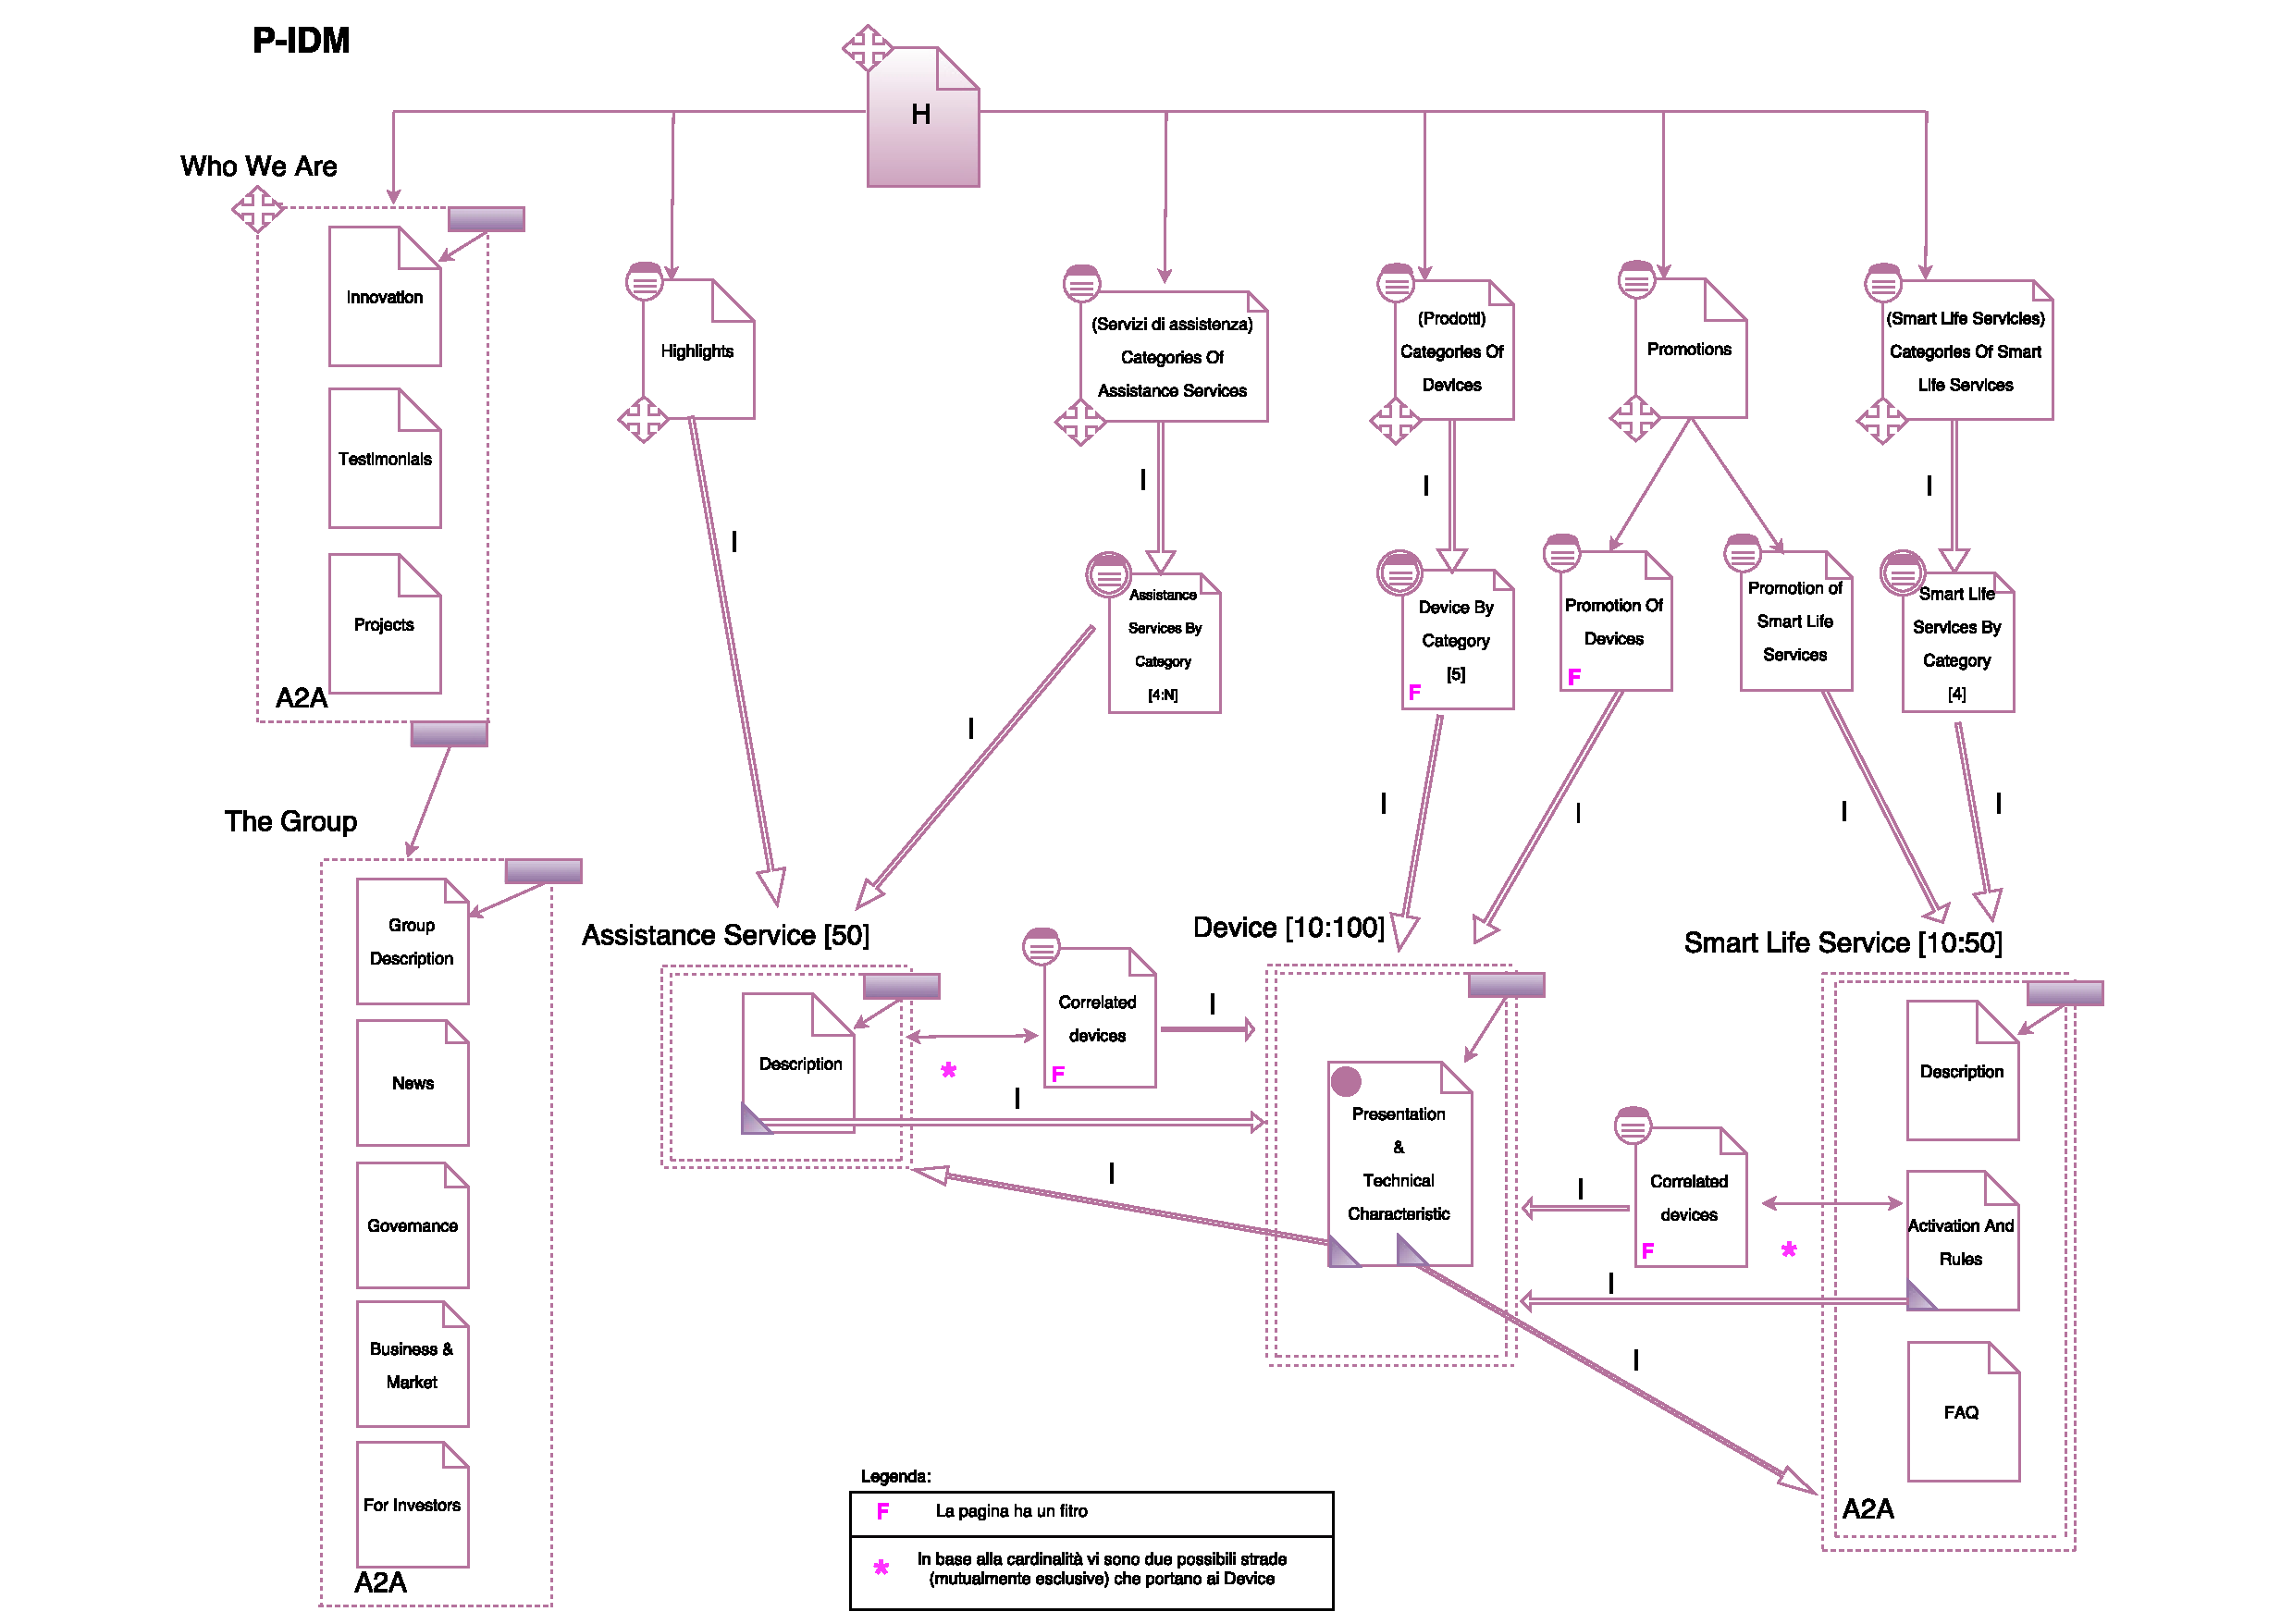
\includepdf[landscape=true, pagecommand={\thispagestyle{empty} \subsection*{}
			\addtocounter{subsection}{1}
			\addcontentsline{toc}{subsection}{\arabic{section}.\arabic{subsection}~~Diagramma P-IDM}}]{Risorse/P-IDM.pdf}
	
	
\end{document}